% Moved from the main text in the scope cut (2026-09-30); text unchanged except cross-references.
\section*{S14. Controlled sweeps, mechanism and theory in detail}
\paragraph{Controlled dermoscopy} With a synthetic ruler whose overlap with the lesion is swept from 0 to 100\% (2,437 ISIC 2018 images, DINOv2
ViT-B/14 at 518\,px, three seeds), ROI masking improves reversed-environment AUROC over ERM by $+0.184$
[$+0.117, +0.250$] when the ruler lies outside the lesion and \emph{lowers} it by $-0.097$ [$-0.164, -0.030$],
$-0.111$ [$-0.181, -0.043$] and $-0.129$ [$-0.195, -0.064$] at 50, 75 and 100\% overlap (location interaction
$+0.313$ [$+0.258, +0.370$]; Table~\ref{tab:synthetic_isic_dino518}); at 25\% overlap the change is not significant
($-0.059$ [$-0.127, +0.008$]). The sign flip is reproduced at 224\,px and
under randomised ruler colour, opacity, ticks and scale. At 0\% overlap the masked model's correlated and reversed
AUROC coincide (0.849/0.849); at 100\% its correlated AUROC exceeds ERM's (0.961 vs 0.937): it uses the ruler
\emph{more}. Synthetic calipers on thyroid nodules, synthetic debris on capsule lesions and synthetic calipers on
ovarian tumours give the same interaction (thyroid $+0.433$ [$+0.362, +0.507$], capsule $+0.228$
[$+0.144, +0.324$], ovary $+0.238$ [$+0.144, +0.340$]; main-text figure of the controlled sweeps); whether the lost benefit becomes harm
depends on the setting (ovary at full overlap $-0.197$ [$-0.357, -0.035$]; thyroid $-0.030$ [$-0.105, +0.042$]).
\begin{table}
\caption{Synthetic ruler, ISIC 2018, DINOv2 ViT-B/14 @518: AUROC and reversed-test Δ vs ERM [95% CI]}
\label{tab:synthetic_isic_dino518}
\begin{tabular}{lllllllllll}
\toprule
Method & Needs & clean@0 & rev@0 & clean@50 & rev@50 & clean@100 & rev@100 & Δrev@0 & Δrev@50 & Δrev@100 \\
\midrule
ERM & — & 0.797 & 0.665 & 0.793 & 0.573 & 0.792 & 0.515 &  &  &  \\
ROI masking & ROI mask (train+test) & 0.849 & 0.849 & 0.829 & 0.476 & 0.825 & 0.386 & +0.184 [+0.146, +0.224] & -0.097 [-0.138, -0.056] & -0.129 [-0.170, -0.087] \\
Inpainting (oracle) & artifact pixels (train+test) & 0.810 & 0.806 & 0.809 & 0.783 & 0.807 & 0.759 & +0.141 [+0.120, +0.162] & +0.211 [+0.187, +0.234] & +0.243 [+0.218, +0.269] \\
Group-balanced & image-level A (train) & 0.814 & 0.802 & 0.815 & 0.792 & 0.806 & 0.796 & +0.137 [+0.109, +0.168] & +0.219 [+0.188, +0.252] & +0.281 [+0.248, +0.315] \\
DFR & image-level A (val) & 0.786 & 0.789 & 0.787 & 0.794 & 0.789 & 0.794 & +0.124 [+0.091, +0.160] & +0.221 [+0.184, +0.261] & +0.279 [+0.240, +0.320] \\
LEACE (paired, oracle renders) & paired renders (train) & 0.829 & 0.832 & 0.810 & 0.810 & 0.809 & 0.809 & +0.167 [+0.139, +0.197] & +0.237 [+0.212, +0.263] & +0.294 [+0.265, +0.325] \\
Repair consistency & artifact pixels (train) & 0.828 & 0.707 & 0.822 & 0.616 & 0.814 & 0.558 & +0.042 [+0.015, +0.069] & +0.043 [+0.014, +0.072] & +0.042 [+0.012, +0.073] \\
I2E (ours) & template library & 0.848 & 0.844 & 0.850 & 0.833 & 0.847 & 0.818 & +0.179 [+0.152, +0.206] & +0.260 [+0.229, +0.291] & +0.303 [+0.271, +0.336] \\
I2E + balanced (ours) & templates + A (train) & 0.841 & 0.842 & 0.843 & 0.840 & 0.844 & 0.842 & +0.177 [+0.151, +0.205] & +0.267 [+0.238, +0.298] & +0.327 [+0.293, +0.362] \\
I2E rank-1 (ablation) & template library & 0.811 & 0.799 & 0.809 & 0.770 & 0.806 & 0.730 & +0.134 [+0.115, +0.154] & +0.197 [+0.174, +0.220] & +0.215 [+0.190, +0.240] \\
Insertion augmentation & template library & 0.814 & 0.726 & 0.812 & 0.654 & 0.810 & 0.603 & +0.061 [+0.049, +0.074] & +0.081 [+0.068, +0.094] & +0.088 [+0.077, +0.099] \\
\bottomrule
\end{tabular}
\end{table}


\paragraph{Mechanism in detail} Three explanations were tested separately. \emph{Occlusion}: with the ruler present but uncorrelated with the
label (50/50), masking changes AUROC by $+0.036$, $+0.041$ and $+0.039$ at 0/50/100\% overlap, none of them
significantly; covering lesion pixels costs nothing measurable, so the harm requires the correlation. \emph{Lost context}: dilating the mask at
50\% overlap \emph{increases} harm ($-0.097 \rightarrow -0.138 \rightarrow -0.153$ for margins 0/10/25\,px; neighbouring
intervals overlap) as the
margin restores ruler pixels (retention $0.50 \rightarrow 0.73 \rightarrow 0.95$); at 100\% overlap, where retention
is already 1, harm is flat ($-0.129$ to $-0.144$) although the ruler's share of visible pixels falls threefold.
\emph{Amplified reliance}: masking doubles the same-head counterfactual sensitivity to the ruler
($|\Delta p|$ 0.235 $\rightarrow$ 0.491 at 100\%). Harm is largest for small lesions ($-0.364$ [$-0.509, -0.217$] at 100\%), where the ruler is a larger share of what
survives the mask; for large lesions the effect at 100\% is not significant ($+0.063$ [$-0.015, +0.144$]), and at 50\%
overlap only the small-lesion stratum is significant, so lesion size orders the harm without defining a threshold.
The main-text mechanism figure shows the same retention mechanism in all five controlled sweeps: with the head held fixed,
inserting the artifact changes the masked model's prediction more the deeper the artifact lies in the ROI. At full
overlap this sensitivity exceeds that of ERM for dermoscopic rulers (0.491 vs 0.235; paired difference $+0.255$
[$+0.221, +0.287$]), ovarian calipers (0.218 vs 0.032; $+0.188$ [$+0.133, +0.250$]) and capsule debris (0.245 vs 0.057;
$+0.186$ [$+0.130, +0.260$]) and matches it for thyroid calipers (0.393 vs 0.369; $+0.025$ [$-0.016, +0.065$]). In chest radiography
ERM ignores a tube outside the lungs ($|\Delta p|=0.005$ at $r=0$), which is why masking has nothing to remove there.
Erasing a generic-overlay subspace after masking and group balancing both lower this sensitivity in every sweep
(S8).

\paragraph{What the real-hair shortcut is made of}
Removing hair pixels at test time only closes 44--47\% of the ERM clean--reversed gap: most of what a frozen
encoder exploits in a real hair trap is not the hair pixels but what accompanies hair (hair-bearing images differ in
sex, age and body site). This bounds every pixel-level method, including oracle inpainting and U-MtE, and
explains why image-level-label methods, which remove everything correlated with the label, recover more.

\paragraph{The linear-Gaussian account: simulation check}
\begin{figure}[H]\centering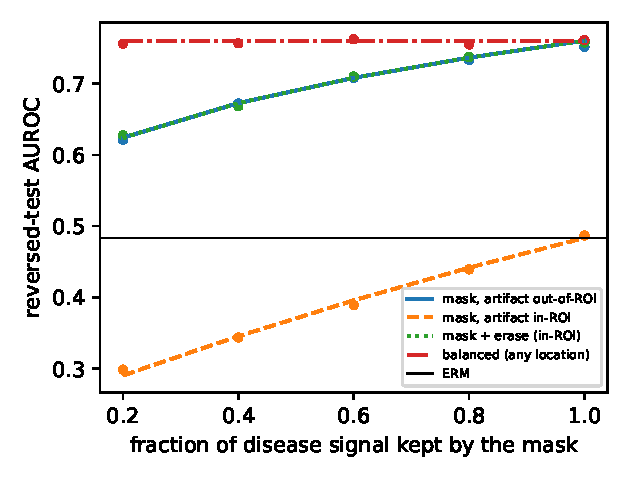
\includegraphics[width=0.6\linewidth]{figures/theory.pdf}
\caption{Reversed-test AUROC predicted by the linear-Gaussian model (lines) and simulated with logistic heads
(points) as masking removes a growing share of disease signal ($S=1$, $A=2$, 90/10 training). Generated by
\texttt{scripts/analysis/theory\_sim.py}.}\label{fig:theory}\end{figure}

\paragraph{Does the account match real encoders?} For any test composition $q_y=P(A{=}1\mid Y{=}y)$ the same head
gives $\mathrm{AUROC}=\Phi\big(\Delta/\sqrt{\sigma_1^2+\sigma_0^2}\big)$ with $\Delta=S+(p_1-p_0)(q_1-q_0)A/(1+vA)$,
$\sigma_y^2=S+w_a^2\,(1+Aq_y(1-q_y))$, $w_a=\sqrt{A}(p_1-p_0)/(1+vA)$ and $v=[p_1(1-p_1)+p_0(1-p_0)]/2$. In a
pre-registered test we fitted $(S,A)$ for every trained model to its clean and correlated AUROC \emph{only} and
compared the implied reversed-test AUROC with the held-out observation; no parameter is shared across models or tuned
(main-text figure of the theory test). Two reference predictors use the same two inputs: ``reversed $=$ clean'' (no
shortcut harm) and a linear-symmetry heuristic, reversed $= 2\cdot$clean $-$ correlated. The endpoint on which the
account is most informative is the held-out reversed-test AUROC itself: over 136 ERM and masking models (real traps
and controlled sweeps) its mean absolute error is 0.052 AUROC ($r=0.91$), against 0.129 for the symmetry heuristic and
0.237 for ``reversed $=$ clean''. Along the controlled overlap sweeps it recovers the sign of the masking gain at 44 of
50 overlap points (symmetry heuristic: 38/50). For the location crossover the gain over the heuristic is small: both
follow the observed crossovers closely across nine cohort--backbone pairs (account: mean absolute error 0.015, 9/9
signs; heuristic: error 0.044, 9/9), because a crossover is a difference of masking gains in which most of the symmetry
already cancels. We therefore do not use the crossover correlation as evidence for the model. The account also matches
end-to-end fine-tuned networks (3/3 crossover signs), which violate its assumptions, and, fitted to DermLIP's clean and
correlated AUROC, it anticipates that encoder's absence of a hair location gap ($+0.013$ implied, $+0.014$ observed;
S18). Adding the chest-radiograph cells (device traps and drains, RAD-DINO; 154 models) leaves the
error almost unchanged (0.053, $r=0.88$), but one near-zero device crossover disagrees in sign (consolidation: observed
$-0.004$, implied $+0.008$; 12 of 13 signs), which fails our pre-registered all-signs criterion, so we call the model a
qualitative account. Its one clear failure is the drain cohort (implied reversed AUROC 0.72--0.78, observed 0.19--0.23):
the clean and correlated environments do not expose a shortcut carried by correlates of the drain, regime~(v).
